\chapter{Implementierung in ROS und Gazebo}
\label{kap5}

Dieses Kapitel stellt eine Implementierung für das in \autoref{kap4} dargestellte Konzept der Entwicklung einer Simulationsumgebung und der Portierung des Algorithmus Random Sampling zur Laufplanung für den Akrobat dar.

\section{Vorgehensweise und Aufbau des Pakets}

Da eine komplette Kopie des vorherigen Algorithmus zur Laufplanung auf Grund verschiedener Umgebungen nicht möglich ist, ist die Vorgehensweise schrittweise wichtige Codestellen zu übertragen und zu testen. Dies hat den Vorteil, dass Funktionen unabhängig voneinander getestet werden können. Damit ergibt sich der folgende Gesamtablauf für die Portierung:
\begin{enumerate}
  \item Aufsetzen der Simulation
  \begin{enumerate}
    \item Aufsetzen des Roboter-Modells
    \item Aufsetzen der Gelenkmotoren
    \item Aufsetzen der Umgebung mittels Gazebo
  \end{enumerate}
  \item Aufsetzen der Fußsteuerung
  \item Testen der Fußsteuerung
  \item Portierung des Laufalgorithmus
\end{enumerate}

Während der Arbeit hat es sich als sinnvoll herausgestellt, die Portierung des Laufplaners erst zum Schluss zu beginnen und mit dem Aufsetzen der Simulation zu beginnen. Der Grund dafür ist, dass es damit während der Portierung möglich ist schon Artefakte in der Simulation zu testen. Damit lässt sich wesentlich besser einschätzen, ob das Übertragene auch funktioniert. Außerdem basiert der Laufplaner auf Funktionalitäten wie dem Roboter-Modell und der Definition der Gelenkmotoren. Mit dieser Vorgehensweise kann das Paket nun schrittweise implementiert werden.

\autoref{Kap4:ROSPackageFolderStructure} definiert die Ordnerstruktur des \ac{ROS}-Pakets. Die Ordnerstruktur ist typisch für \ac{ROS}-Pakete und findet sich ähnlich in vielen weiteren Paketen der \ac{ROS}-Community. Der Aufbau des Pakets ist an das Akrobat-Paket \autocite{akrobat} sowie das Hopper-Paket \autocite{hopper} angelehnt. Beide Pakete nutzen wichtige Konzepte für das Robotermodelle und die Gelenksteuerung, die auch für dieses Projekt wichtig sind.

\begin{figure}[p!]
\dirtree{%
.1 hexapod.
.2 config.
.3 config.rviz.
.3 hexapod.yaml.
.2 urdf.
.3 hexapod.xacro.
.3 leg-1.xacro.
.3 leg-2.xacro.
.3 leg-3.xacro.
.3 leg-4.xacro.
.3 leg-5.xacro.
.3 leg-6.xacro.
.2 launch.
.3 rviz.launch.
.3 gazebo.launch.
.3 model.launch.
.3 akrobat\_walk.launch.
.3 control.launch.
.2 include.
.3 akrobat.
.4 akrobat\_init.h.
.4 JointStateToGazebo.h.
.4 ControlRandomSampling.h.
.4 JointStateToDynamixel.h.
.4 FootConfiguration.h.
.4 Akrobat.h.
.3 pugixml.
.2 worlds.
.3 default.world.
.2 stl.
.3 hexapod\_link.stl.
.3 coxa\_r\_link.stl.
.3 coxa\_l\_link.stl.
.3 femur\_link.stl.
.3 tibia\_link.stl.
.2 src.
.3 akrobat.
.4 akrobat\_main.cpp.
.4 JointStateToGazebo.cpp.
.4 FootConfiguration.cpp.
.4 JointStateToDynamixel.cpp.
.4 Akrobat.cpp.
.4 ControlRandomSampling.cpp.
.3 pugixml.
}
\caption{Dateibaum des ROS-Pakets}
\label{Kap4:ROSPackageFolderStructure}
\end{figure}

\section{Aufsetzen der Simulation}

Das erste Ziel ist es nun, den Akrobat in Gazebo anzuzeigen. Dazu muss das Robotermodell integriert werden, die Gelenkmotoren definiert werden und die Gazebo-Welt aufgesetzt werden.

\subsection{Aufsetzen des Robotermodells mittels URDF}

Als erstes wird das Robotermodell in das neue \ac{ROS}-Paket integriert. Die vorliegende Roboterbeschreibung liegt im \ac{URDF}-Format vor. Des Weiteren existieren die 3D-Modelle im \emph{stl}-Format, welche im Robotermodell eingebunden sind. Damit das Robotermodell auch bei späteren Änderungen noch wartbar bleibt, wird die zusammenhängende Datei in das \ac{Xacro}-Format umgebaut, so dass nun eine Datei für die Robotermitte und eine Datei für jedes einzelne Bein existiert. Mit diesem Aufbau könnte das Robotermodell nun schon über ein Launch-File im 3D Visualisierungs-Tool "`rviz"' angezeigt werden. \autoref{Kap4:AkrobatRviz} zeigt stellt dies sowie die Koordinatensystemen des Roboters dar.

\begin{figure}[b!]
  \centering
  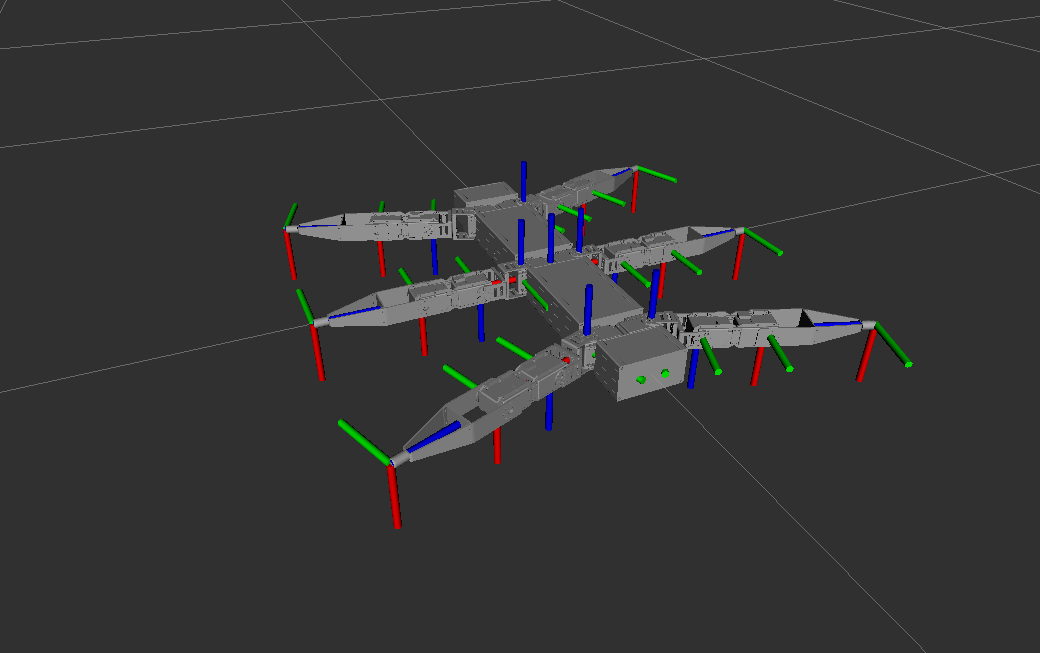
\includegraphics[height=8cm]{kapitel4/akrobat-rviz}
  \caption{Darstellung des Akrobats im rviz}
  \label{Kap4:AkrobatRviz}
\end{figure}

Für das spätere Hinzufügen des Akrobats in die \emph{Gazebo}-Simulation müssen neben der Visualisierung, die für den rviz ausreichend war, noch weitere Anpassungen am Roboter-Modell vorgenommen werden:
\begin{itemize}
  \item Aufsetzen des Kollisionsmodells durch das Attribut <collission>
  \item Aufsetzen der Massenschwerpunkte und der Trägheitsmomente durch das Attribut <inertia>
\end{itemize}

Danach ist das statische Modell fertig aufgesetzt. Nun müssen die Gelenkmotoren an den Gelenken definiert werden, damit diese von \ac{ROS} angesteuert werden können.

\subsection{Definition der Gelenkmotoren mittels ros\_control}

Das zuvor aufgesetzte Robotermodell könnte nun in Gazebo angezeigt werden. Allerdings ist dieses noch nicht durch Eingaben von außen beweglich, da keine Gelenkmotoren definiert sind. Diese werden in diesem Abschnitt behandelt.

Hierbei hat sich das Paket \emph{ros\_control} als geeignet herausgestellt. Für das Aufsetzen des Pakets wird eine Konfigurationsdatei für die Definition aller Controller benötigt. Außerdem muss im Robotermodell ein Gelenk auf einen Controller abgebildet werden, damit das Gelenk angesteuert werden kann. Außerdem müssen zwei wesentliche Plugins eingebunden und konfiguriert werden:
\begin{itemize}
  \item gazebo\_ros\_control
  \item p3d\_base\_controller
\end{itemize}

Abschließend muss die Konfigurationsdatei geladen und zwei \ac{ROS}-Nodes gestartet werden. Dies ist zum einen der \emph{robot\_state\_publisher}, der die publizierten Bewegungen an den Roboter weitergibt, sowie ein \emph{controller\_manager}, der letztendlich die einzelnen Gelenke in der Simulation bewegt. Hier lässt sich statt dem \emph{controller\_manager} auch direkt ein \emph{dynamixel\_manager} anbinden, so dass später leicht zwischen Simulation und dem realen Roboter gewechselt werden kann. Durch die Einbindung existieren nun zur Laufzeit einige wichtige \ac{ROS}-Topics, wie in \autoref{Kap4:RosControlTopics} zu sehen ist.

\begin{figure}[p!]
  \centering
  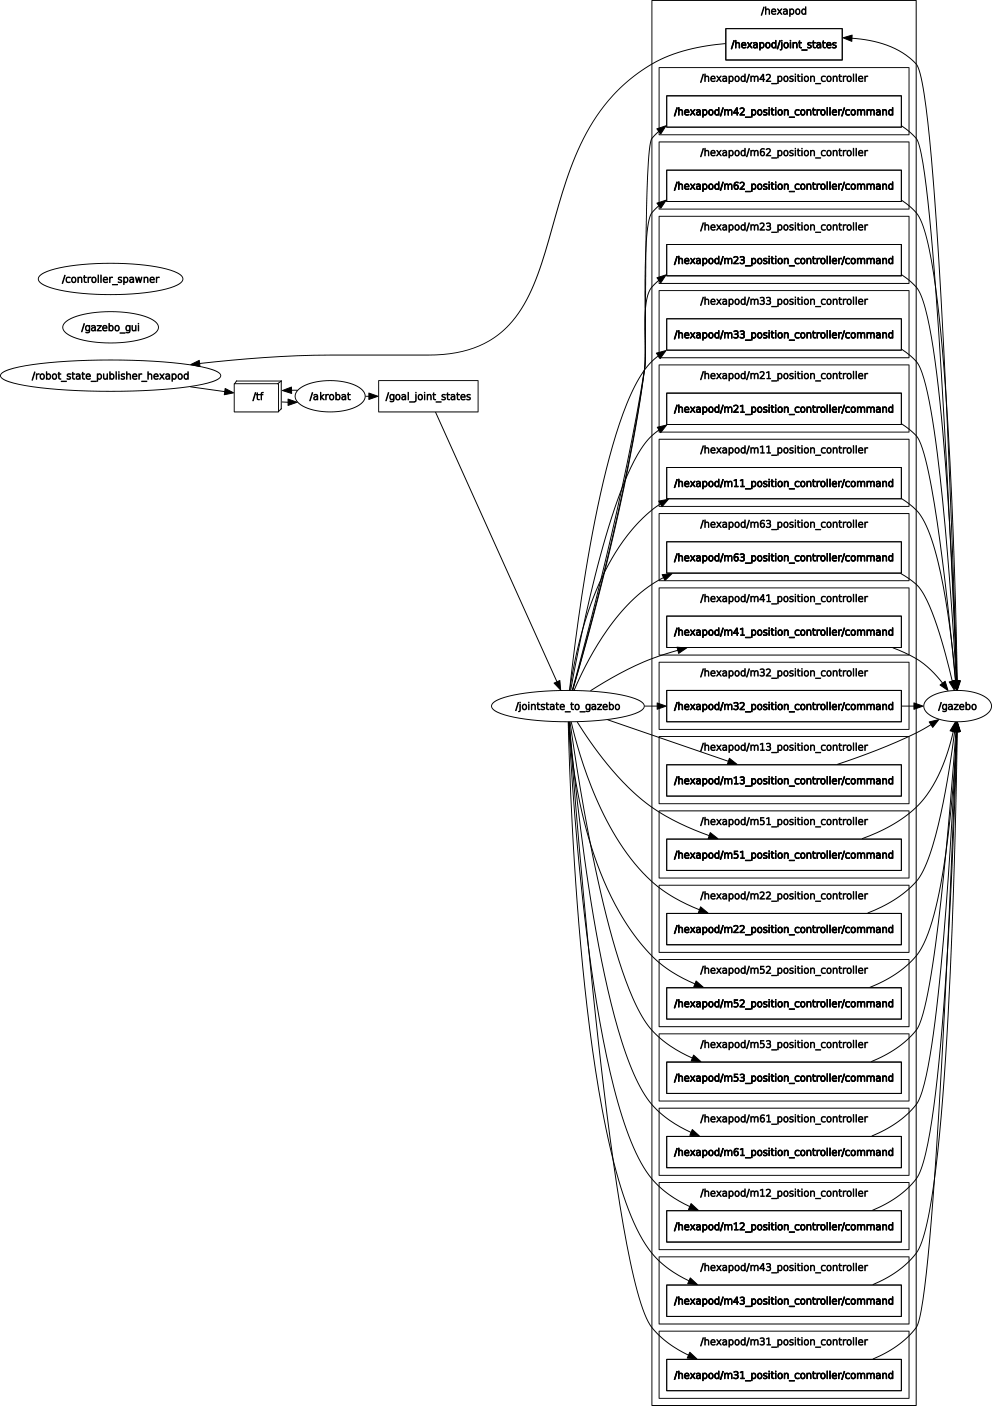
\includegraphics[height=23cm]{kapitel4/rosgraph}
  \caption{ROS-Topics der Simulation}
  \label{Kap4:RosControlTopics}
\end{figure}

\subsection{Aufsetzen der Umgebung mittels Gazebo}

Nun fehlt nur noch die Gazebo-Umgebung. Diese lässt sich mit einem von Gazebo bereitgestellten Launch-File starten. Es besteht die Möglichkeit Parameter mitzugeben. Die folgende Auflistung beschreibt einige wichtige Parameter:
\begin{itemize}
  \item \emph{world\_name}: Dateipfad zur gewünschten Welt
  \item \emph{debug}: Gibt Informationen zur Analyse während der Laufzeit aus
  \item \emph{gui}: Startet die grafische Oberfläche
  \item \emph{paused}: Pausiert die Simulation
\end{itemize}

Damit ist das Aufsetzen des Roboters sowie der Simulationsumgebung vollständig. Der Roboter wird nun in Gazebo angezeigt, wie in \autoref{kap4:gazeboflach} zu sehen ist.

\section{Aufsetzen der Ausgangsposition}

Der Roboter wird nun zwar im Gazebo angezeigt, allerdings liegt dieser nun flach auf dem Boden. Das Ziel ist es daher, die Fußsteuerung aufzusetzen, so dass der Roboter sich zu Beginn in seine Ausgangsstellung begibt. Von dort aus wartet der Roboter auf weitere Befehle für die Bewegung.

\begin{figure}[b!]
  \centering
  \begin{subfigure}[b]{.4\linewidth}
    \centering
    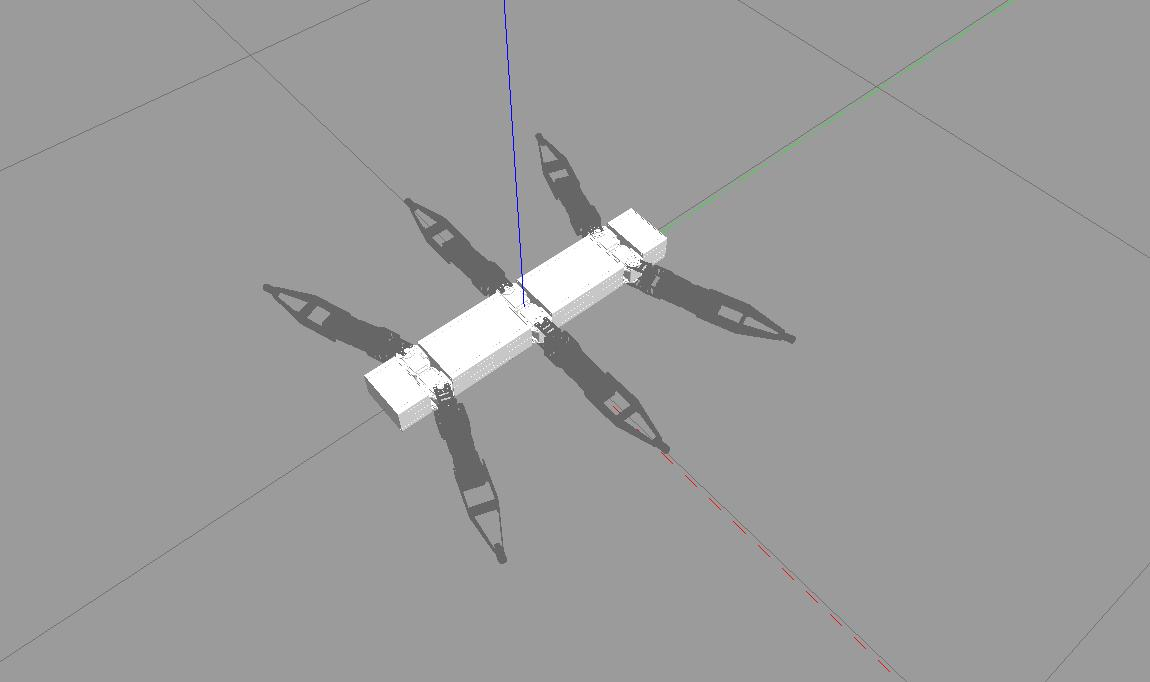
\includegraphics[width=6cm]{kapitel4/akrobat-flach}
    \subcaption{Vor Aufsetzen der Ausgangsposition}\label{kap4:gazeboflach}
  \end{subfigure}%
  \qquad
  \begin{subfigure}[b]{.4\linewidth}
    \centering
    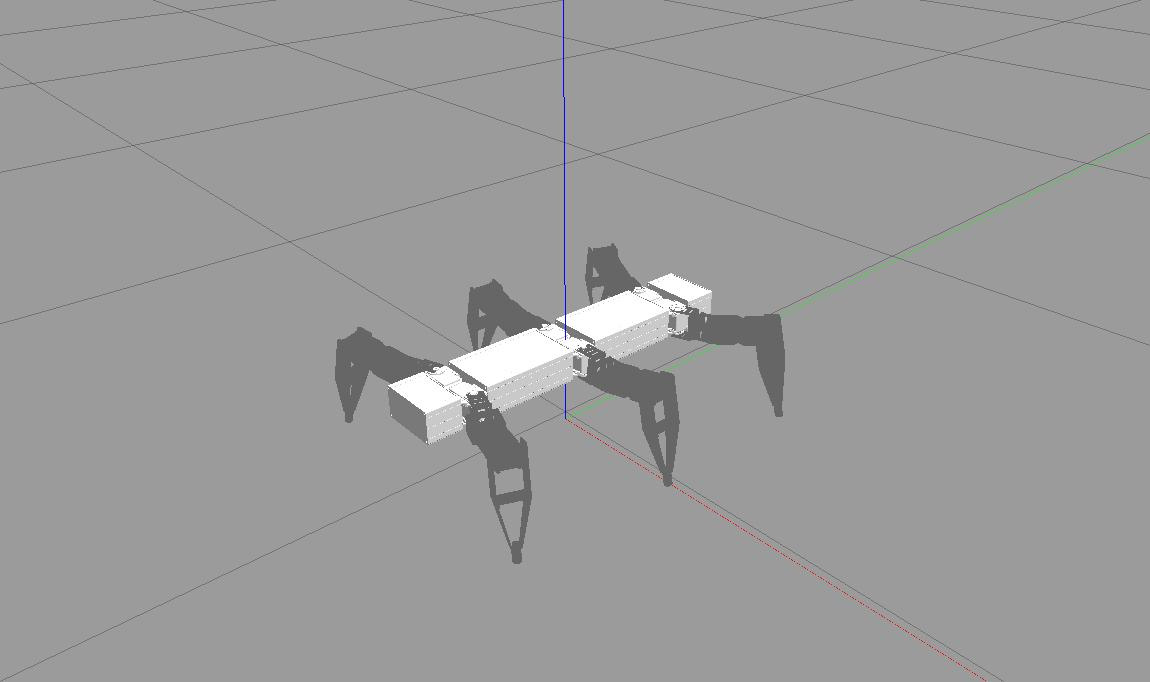
\includegraphics[width=6cm]{kapitel4/akrobat-oben}
    \subcaption{Nach Aufsetzen der Ausgangsposition}\label{kap4:gazebooben}
  \end{subfigure}\\
  \caption{Aufstehen des Akrobat in Gazebo}
  \label{kap4gazebo}
\end{figure}

Da \ac{ROS}-Nodes allgemein in einer Schleife laufen, wird der folgende Ablauf kontinuierlich ausgeführt. Der Ablauf sorgt wie in \autoref{kap4:gazebooben} zu sehen, dafür, dass der Roboter in den nächsten Durchläufen in der Ausgangsposition steht. Dies erfolgt in mehreren Schritten: 
\begin{enumerate}
  \item Zunächst wird über das \textsc{tf}-Framework} mit Hilfe von Transformationen und Rotationen die Ausgangsposition vom obersten Gelenk zum Endeffektor berechnet. Dies wird im weiteren Verlauf als Ausgangsposition definiert und eingelesene Bewegungen sind relativ zu dieser Position.
  \item Die dazugehörigen Winkel, die benötigt werden, um in die Ausgangsposition zu kommen, werden nun mittels \emph{inverser Kinematik} berechnet.
  \item Die drei Winkel werden nun in das Topic \emph{goal\_joint\_states} geschrieben, was ein tatsächliches Verändern der Winkel in der Simulation oder am echten Roboter verursacht. Dabei wird vorher geprüft, ob die Winkel gültig sind, d.h. dass sie sich über dem minimal und unter dem maximal erlaubten Winkel befinden. Ist das nicht der Fall, wird eine Warnung ausgegeben.
\end{enumerate}

\section{Generieren und Einlesen von Bewegungen als xml-Datei}

Die Generierung erfolgt durch die Iteration über die von einem Algorithmus generierten Schritte für die Fußpositionen. Statt für die Generierung eine xml-Bibliothek zu nutzen, reicht hier eine einfache Ausgabe in einer Datei mittels \emph{ofstream}.

\autoref{lst:MovementExample} zeigt eine abgespeckte XML-Bewegung der ersten beiden Füße, welche den Fuß an der 1. Stelle ein wenig in $y$-Richtung verschieben würde, was einer Verschiebung der Robotermitte verursacht, sofern die anderen Füße, welche auf dem Boden sind, das auch tun. Des Weiteren wird der Fuß an der 2. Stelle ein Stück angehoben.

Für das Einlesen der XML-Datei wird Pugixml \autocite{pugixml} verwendet, welches unkompliziert und schnell xml-Dateien generieren oder einlesen kann. Die eingelesene Bewegung wird als Vektor in C++ gespeichert und an den Akrobat weitergegeben. Dieser ist dann für das Abspielen der Bewegung zuständig.

\lstinputlisting[language=Xml,caption={Aufbau der Bewegungsdatei},label=lst:MovementExample,float=t!]{\srcloc/movement-1.xml}

\section{Abspielen der Bewegungen}

Das \ac{ROS} läuft in einer Schleife, bei der die Periode definiert werden kann. Als geeignet hat sich ein Wert von 20 Millisekunden herausgestellt. Auf Grund der Tatsache, dass die xml-Datei keine Bewegungsdauern speichert, muss eine Synchronisation zwischen dem \ac{ROS}-Loop und dem Abspielen der Bewegung aufgesetzt werden. Damit die Bewegungen nicht unrealistisch aussehen und linear von Position zu Position wechseln, wird eine Interpolation zwischen den einzelnen Punkten mittels einer trigonometrischen Funktion aufgesetzt.
\begin{eqnarray}
\label{kap4:cosinterpolation}
f(x) = -0,5 \cdot \cos{(x)} + 0{,}5 \\
\label{kap4:cosinterpolation2}
f(y) = -0,5 \cdot \cos{(y)} + 0{,}5 \\
\label{kap4:cosinterpolation3}
f(z) = -0,5 \cdot \cos{(z)} + 0{,}5
\end{eqnarray}

Der in \autoref{kap4:cosinterpolation}, \ref{kap4:cosinterpolation2} sowie \ref{kap4:cosinterpolation3} verwendete Cosinus ist skaliert und vertikal verschoben, so dass er von 0 bis 1 reicht. Geht man davon aus, dass eine Bewegung in acht Durchläufen der Schleife abgelaufen sein soll, ergibt sich also für eine Bewegung eine Zeitdauer von mindestens 160 Millisekunden. Diese Zahl kann weiter optimiert werden, so dass die maximale Geschwindigkeit der Beinregler nicht überschritten wird. Die Simulation lässt sich mit diesem Wert allerdings sehr gut testen.

Code-technisch ist das mit drei Variablen umgesetzt, die die aktuelle Zwischenposition bestimmen. Die erste Variable gibt die maximale Zahl der Zwischenpositionen an (\emph{maxTicks}). Die zweite Variable gibt die aktuelle Stelle (\emph{tick}) an, so dass der Algorithmus über die Funktion ausrechnen kann, was die nächste Position sein wird. Die Variable \emph{diff} ist der Vektor von der Start- zur Zielposition. \autoref{interpolationZwischenwerte} zeigt die vollständige Berechnung einer Zwischenposition.

\begin{lstlisting}[label={interpolationZwischenwerte}, language=C++, caption={Interpolation der Zwischenpositionen}]
double x = diff.x() * (-0.5 * cos(M_PI * tick / maxTicks) + 0.5);
double y = diff.y() * (-0.5 * cos(M_PI * tick / maxTicks) + 0.5);
double z = diff.z() * (-0.5 * cos(M_PI * tick / maxTicks) + 0.5);
\end{lstlisting}

In jedem Schritt wird der \emph{tick} um eins nach oben gesetzt, bis er bei der Grenze von \emph{maxTicks} angekommen ist. Dann wird dieser zurückgesetzt und die nächste Bewegung wird ausgeführt.

\section{Aufsetzen des Dreifußgangs}

Bevor das Random Sampling aufgesetzt wird, ist es sinnvoll die gesamte Simulation zunächst mit einem statischen Laufmuster zu prüfen. Das macht es später einfacher zwischen einem Fehler in der Simulation und einem Fehler in der Laufplanung zu unterscheiden.

Beim Dreifußgang kann ein Fuß einen von zwei Stati annehmen:
\begin{enumerate}
  \item Der Fuß wird angehoben und umgesetzt.
  \item Der Fuß ist für das Verschieben der Körpermitte verantwortlich.
\end{enumerate}

Zunächst werden die Stati für jeden Fuß in einem Array in C++ gesetzt. Die Füße 1, 4 und 5 starten in der ersten Phase, die Füße 2, 3 und 6 starten in der zweiten Phase. Mit jeder Bewegung wird dies abgewechselt sowie die Positionen relativ zum Fußpunkt gesetzt. Für Phase 1 muss die $z$-Koordinate positiv gesetzt werden, damit der Fuß angehoben wird. In Phase 2 muss die $z$-Koordinate auf null gesetzt werden, damit der Fuß die Körpermitte verschieben und stützen kann sowie die Position ein wenig nach hinten verschoben werden, damit der Körper sich nach vorne bewegt. Die stützenden Füße sind so gewählt, dass der Stability Margin größer als null ist, damit der Roboter nicht umkippt. Das Ergebnis wird als Bewegungsdatei exportiert und kann vom Roboter eingelesen werden.

\section{Aufsetzen des Random Samplings}

Wie auch bei den Vorgängern ist die Implementierung mit C++ durchgeführt. Im folgenden Abschnitt werden einige wesentliche Unterschiede bei der Implementierung dargestellt.

\subsection{Abstrahierung der Fußkonfiguration}

Während bei dem vorherigen Laufplaner die aktuelle Fußkonfiguration und die Fußposition getrennt voneinander gespeichert wurden, speichert der neue Laufplaner diese in dem Klassenobjekt \emph{FootConfiguration}. Dies hat den Vorteil, dass diese gesamte Fußlogik in einer Klasse gekapselt und unabhängig vom Laufplaner getestet werden könnte.

Außerdem macht dies das Debugging einfacher, da sich in einer gekapselten Klasse beispielsweise Methoden zur Ausgabe definieren lassen. Dadurch lassen sich auch einige redundante Code-Zeilen sparen, da wiederkehrende Funktionen abstrahiert werden.

\subsection{Nutzung des \textsc{tf}-Frameworks und Anpassung aller Maße}

Alle 2D und 3D-Berechnungen werden nun mit dem \textsc{tf}-Framework aus \ac{ROS} berechnet. Dieses speichert alle Längenangaben in Meter. Da die OpenInventor-Simulation alle Angaben in Millimeter gespeichert hat, muss der Algorithmus ebenfalls Meterangaben liefern.

Des Weiteren müssen weitere definierte Angaben verändert werden:
\begin{itemize}
  \item Angepeilte Zielposition des Roboters
  \item Schrittgröße als potentielle Position für das Absetzen des Fußes 
  \item Abschnittslänge für die spiralförmige Suche beim Absetzen des Fußes
  \item Minimal gültiger Stability-Margin
  \item Maximale Anzahl von Anhebungen oder Absetzungen von Füßen
\end{itemize}

\subsection{Veränderung der Zufallszahlengenerierung}

Für die Generierung von Zufallszahlen steigt das System auf den Pseudozufallszahlengenerator Mersenne-Twister \autocite{matsumoto1998mersenne} um. Außerdem wird beispielsweise die geometrische Verteilung nicht mehr selbst programmiert, sondern mit einer existierenden Funktion über den Pseudozufallszahlengenerator geregelt, die dies bereits implementiert. Der Aufruf erfolgt über die Standardbibliothek wie in \autoref{geometricDistribution}.

\begin{lstlisting}[label={geometricDistribution}, language=C++, caption={Geometrische Verteilung mittels C++}]
std::random_device rd;
std::mt19937 generator(rd());
std::geometric_distribution<int> geometricDistribution(0.5);

int result = randomDistribution(generator);
\end{lstlisting}